% ----------------------------------------------------------------------
% Capítulo: Materiais e Métodos
%
% Neste capítulo descrevem‑se os dados, a metodologia estatística e os
% procedimentos analíticos utilizados. Segue as normas de numeração
% progressiva das seções e subseções.

\chapter{Material e métodos}
\section{Fontes e coleta de dados}

Todo o desenvolvimento computacional deste estudo foi realizado utilizando o 
software R (versão 4.5.1)\cite{rsoftware}. Além disso, os dados de interesse 
foram extraídos por meio do pacote \texttt{microdatasus}\cite{saldanha2019microdatasus}. 
A seguir, são detalhadas as bases de dados utilizadas e os procedimentos metodológicos 
adotados.

\subsection{Sistema de Informações sobre Mortalidade - Declaração de Óbitos
Fetais (SIM-DOFET)}

Os dados públicos de mortalidade no Brasil são disponibilizados pelo Sistema de 
Informações sobre Mortalidade (SIM) \cite{DATASUSSIM2023}. Especificamente, os óbitos fetais são 
registrados em uma extensão do SIM para declarações de óbitos fetais 
(SIM-DOFET), no qual os casos são incluídos de acordo com critérios padronizados 
pelo Ministério da Saúde. De forma geral, óbito fetal é definido como a morte do 
produto da concepção antes da expulsão ou extração completa do corpo materno, 
independentemente da duração da gestação, na ausência de qualquer sinal de vida 
após a separação, como respiração, batimentos cardíacos, pulsações do cordão 
umbilical ou movimentos musculares voluntários efetivos \cite{Andrade2005,Lawn2016}. 
No Brasil, recomenda-se o preenchimento da Declaração de Óbito Fetal para perdas 
gestacionais com idade gestacional igual ou superior a 20 semanas, peso fetal igual 
ou superior a 500 gramas ou estatura igual ou superior a 25 centímetros \cite{Andrade2005,ministerioSaudeDO2022}. 
Entretanto, como a base do SIM-DOFET utilizada neste estudo não dispõe de informação 
sobre a estatura, a definição adotada considera como óbito fetal os registros que 
atenderam aos critérios para idade gestacional e peso fetal definidos.

A Figura \ref{fig:fluxograma-sim} apresenta o fluxograma do processo de seleção
dos registros até a obtenção da base de óbitos fetais no ano de 2023, no estado
de São Paulo e sem dados faltantes nas variáveis de interesse, totalizando 3.266
óbitos fetais para análise.

%------------------------ Fluxograma SIM-DOFET
\begin{figure}[H]
  \centering
  \caption{Fluxograma das etapas de filtragem e obtenção dos dados de óbitos
  fetais utilizados no estudo.}
  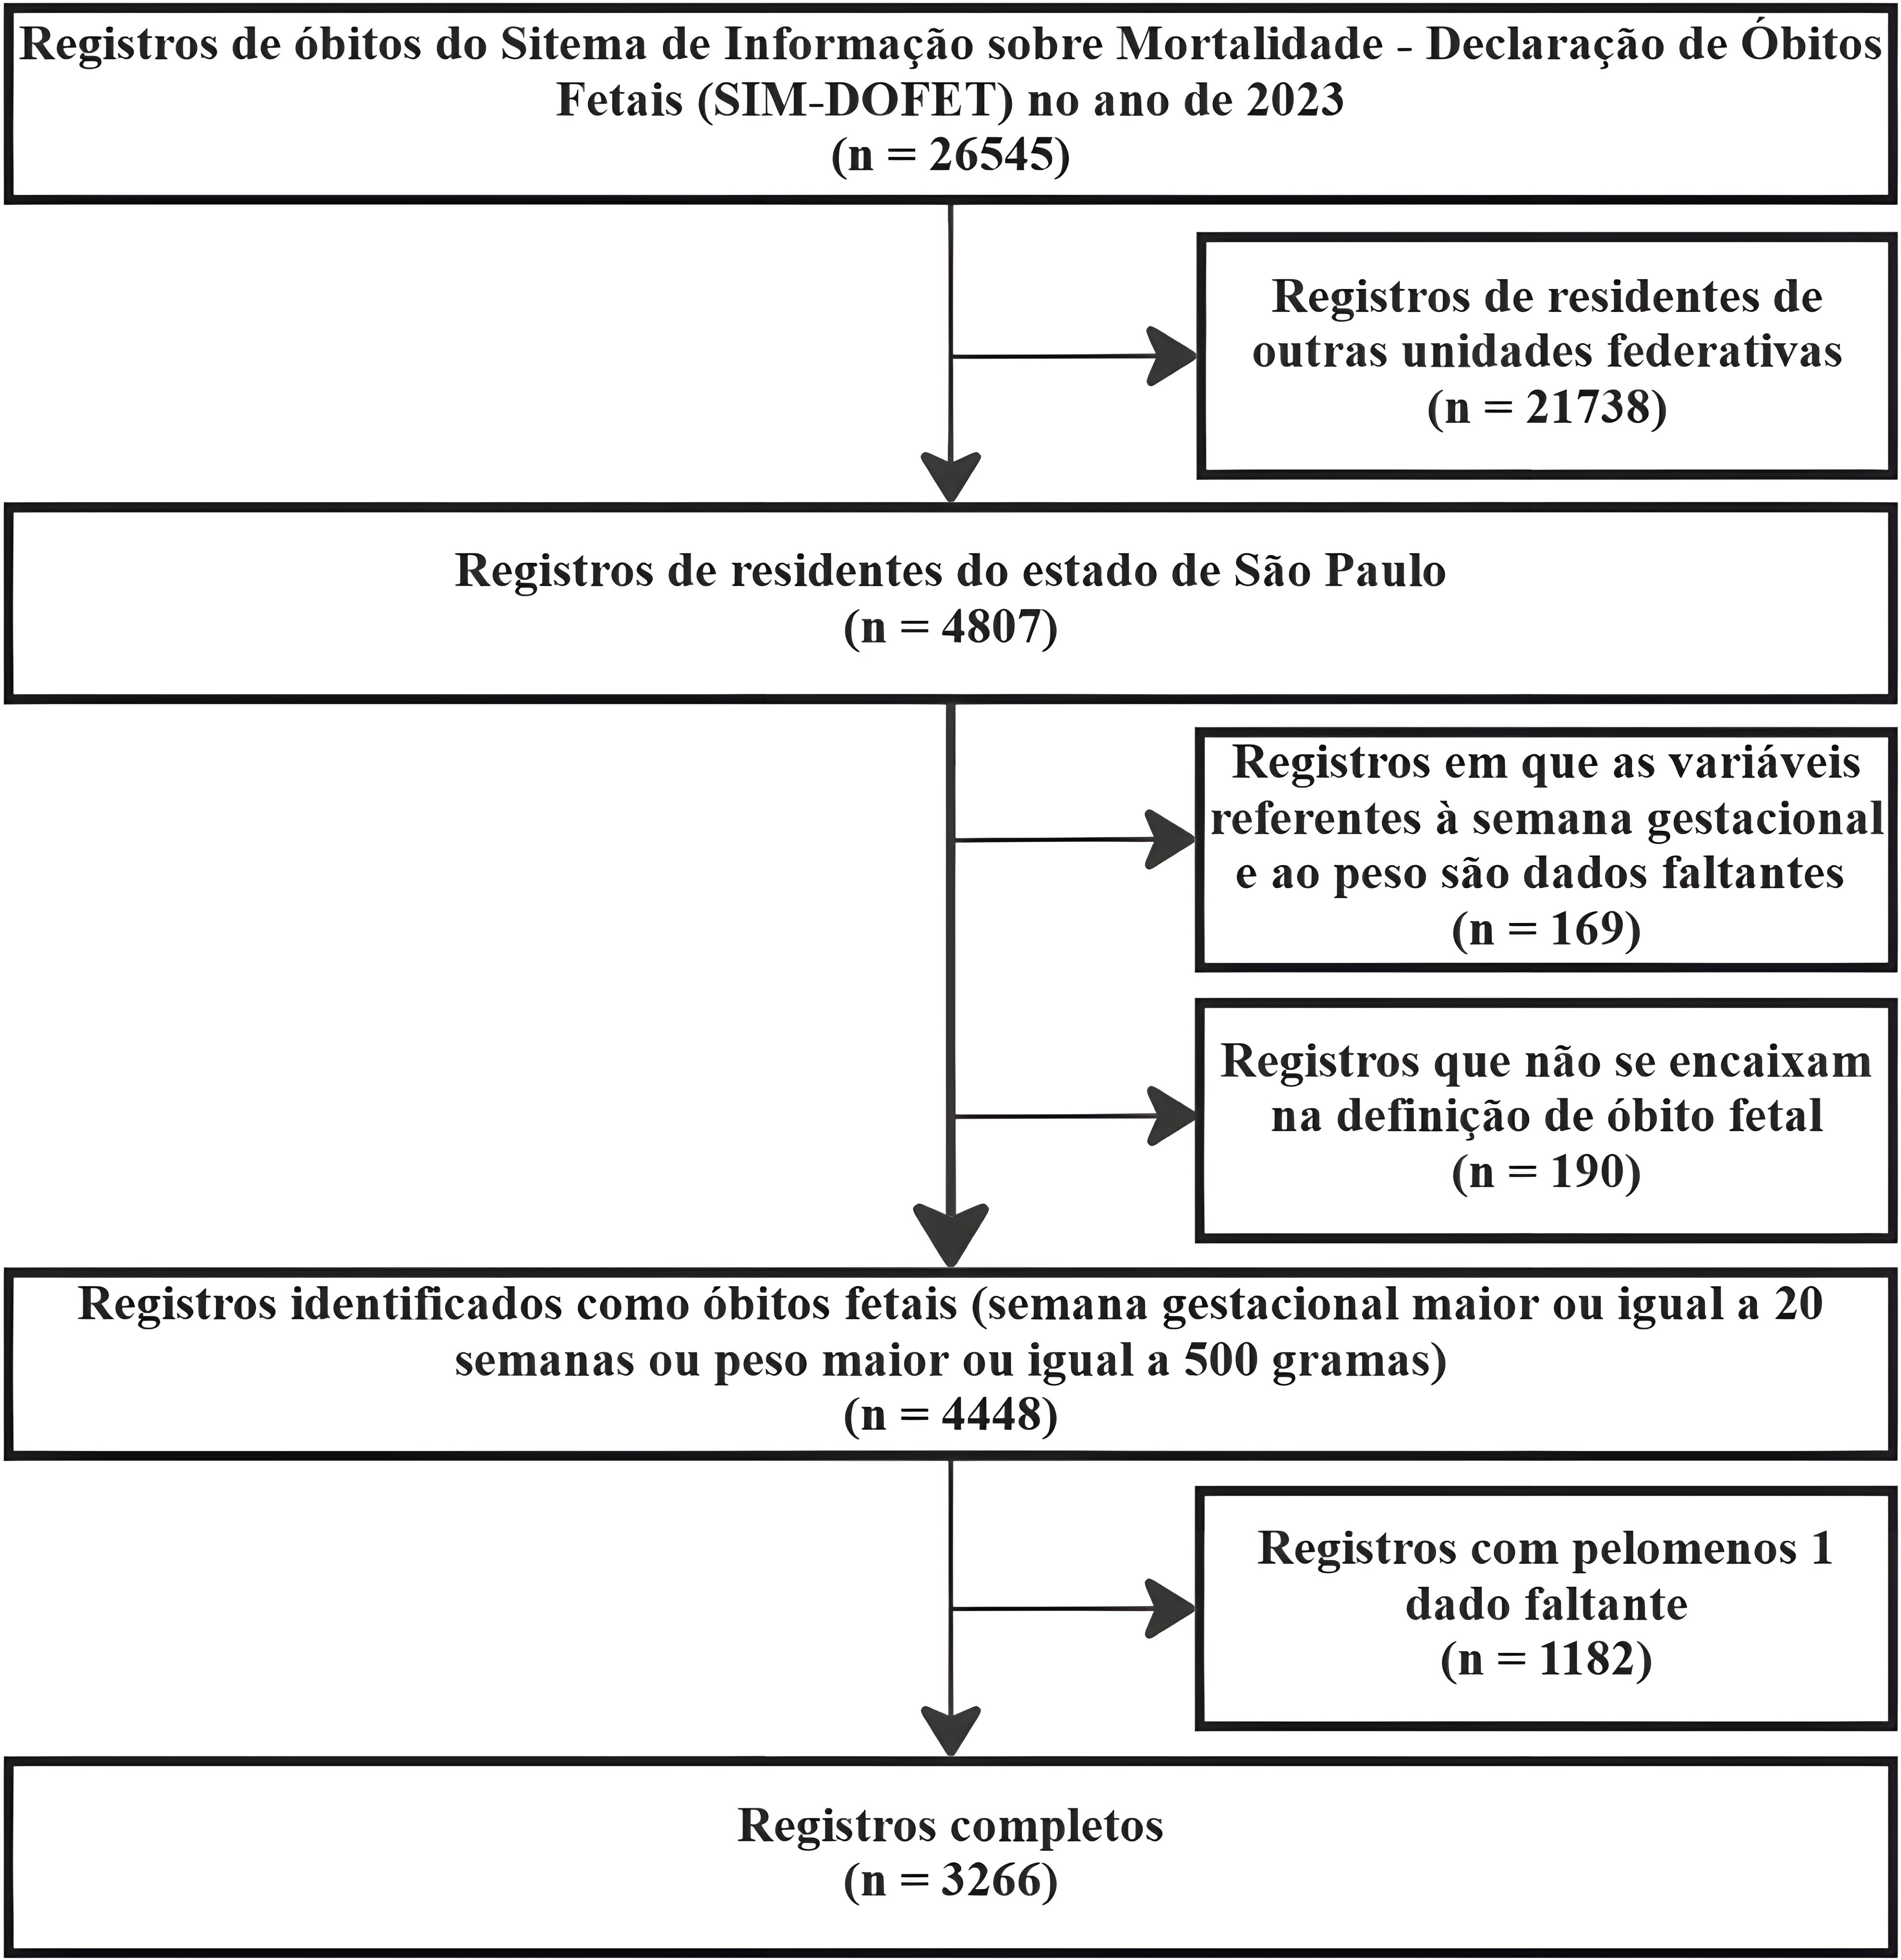
\includegraphics[width=0.8\linewidth]{figuras/flux_obitos_fetais.png}
  \fonte{Fonte: figura elaborada pelo autor.}
  \label{fig:fluxograma-sim}
\end{figure}

%------------------------ Fluxograma SINASC
\subsection{Sistema de
Informações sobre Nascidos Vivos (SINASC)}

Os dados de nascidos vivos são disponibilizados por meio do Sistema de
Informações sobre Nascidos Vivos (SINASC) \cite{DATASUSSINASC2023}, o qual é alimentado pela Declaração de 
Nascido Vivo (DNV). Para fins de registro, nascimento vivo é definido como a 
expulsão ou extração completa do produto da concepção do corpo materno que, 
após a separação, apresenta respiração ou qualquer outro sinal de vida, como 
batimentos cardíacos, pulsação do cordão umbilical ou movimentos musculares 
voluntários, independentemente da duração da gestação \cite{ministerioSaudeDNV2022}. 
No contexto deste estudo, em que o interesse é o tempo até o parto, gestações que
resultam em nascimento vivo do feto são caracterizadas como evento competidor 
\cite{satagopan2004note,naimi2016cumulative}. Isso ocorre porque, uma vez 
desencadeado o óbito fetal, torna-se impossibilitada a ocorrência de nascimento 
vivo. De forma análoga, se o desfecho observado primeiro é o nascimento vivo, o 
óbito fetal passa a ser impossibilitado, independentemente do tempo de observação 
do caso.

A Figura \ref{fig:fluxograma-sinasc} apresenta o fluxograma das etapas de processamento 
da base de dados, considerando os registros de 2023 para o estado de São Paulo e 
sem dados faltantes nas variáveis de interesse, totalizando 485.922 nascimentos 
vivos válidos.

\begin{figure}[H]
  \centering
  \caption{Fluxograma das etapas de filtragem e obtenção dos dados de nascidos
  vivos utilizados no estudo.}
  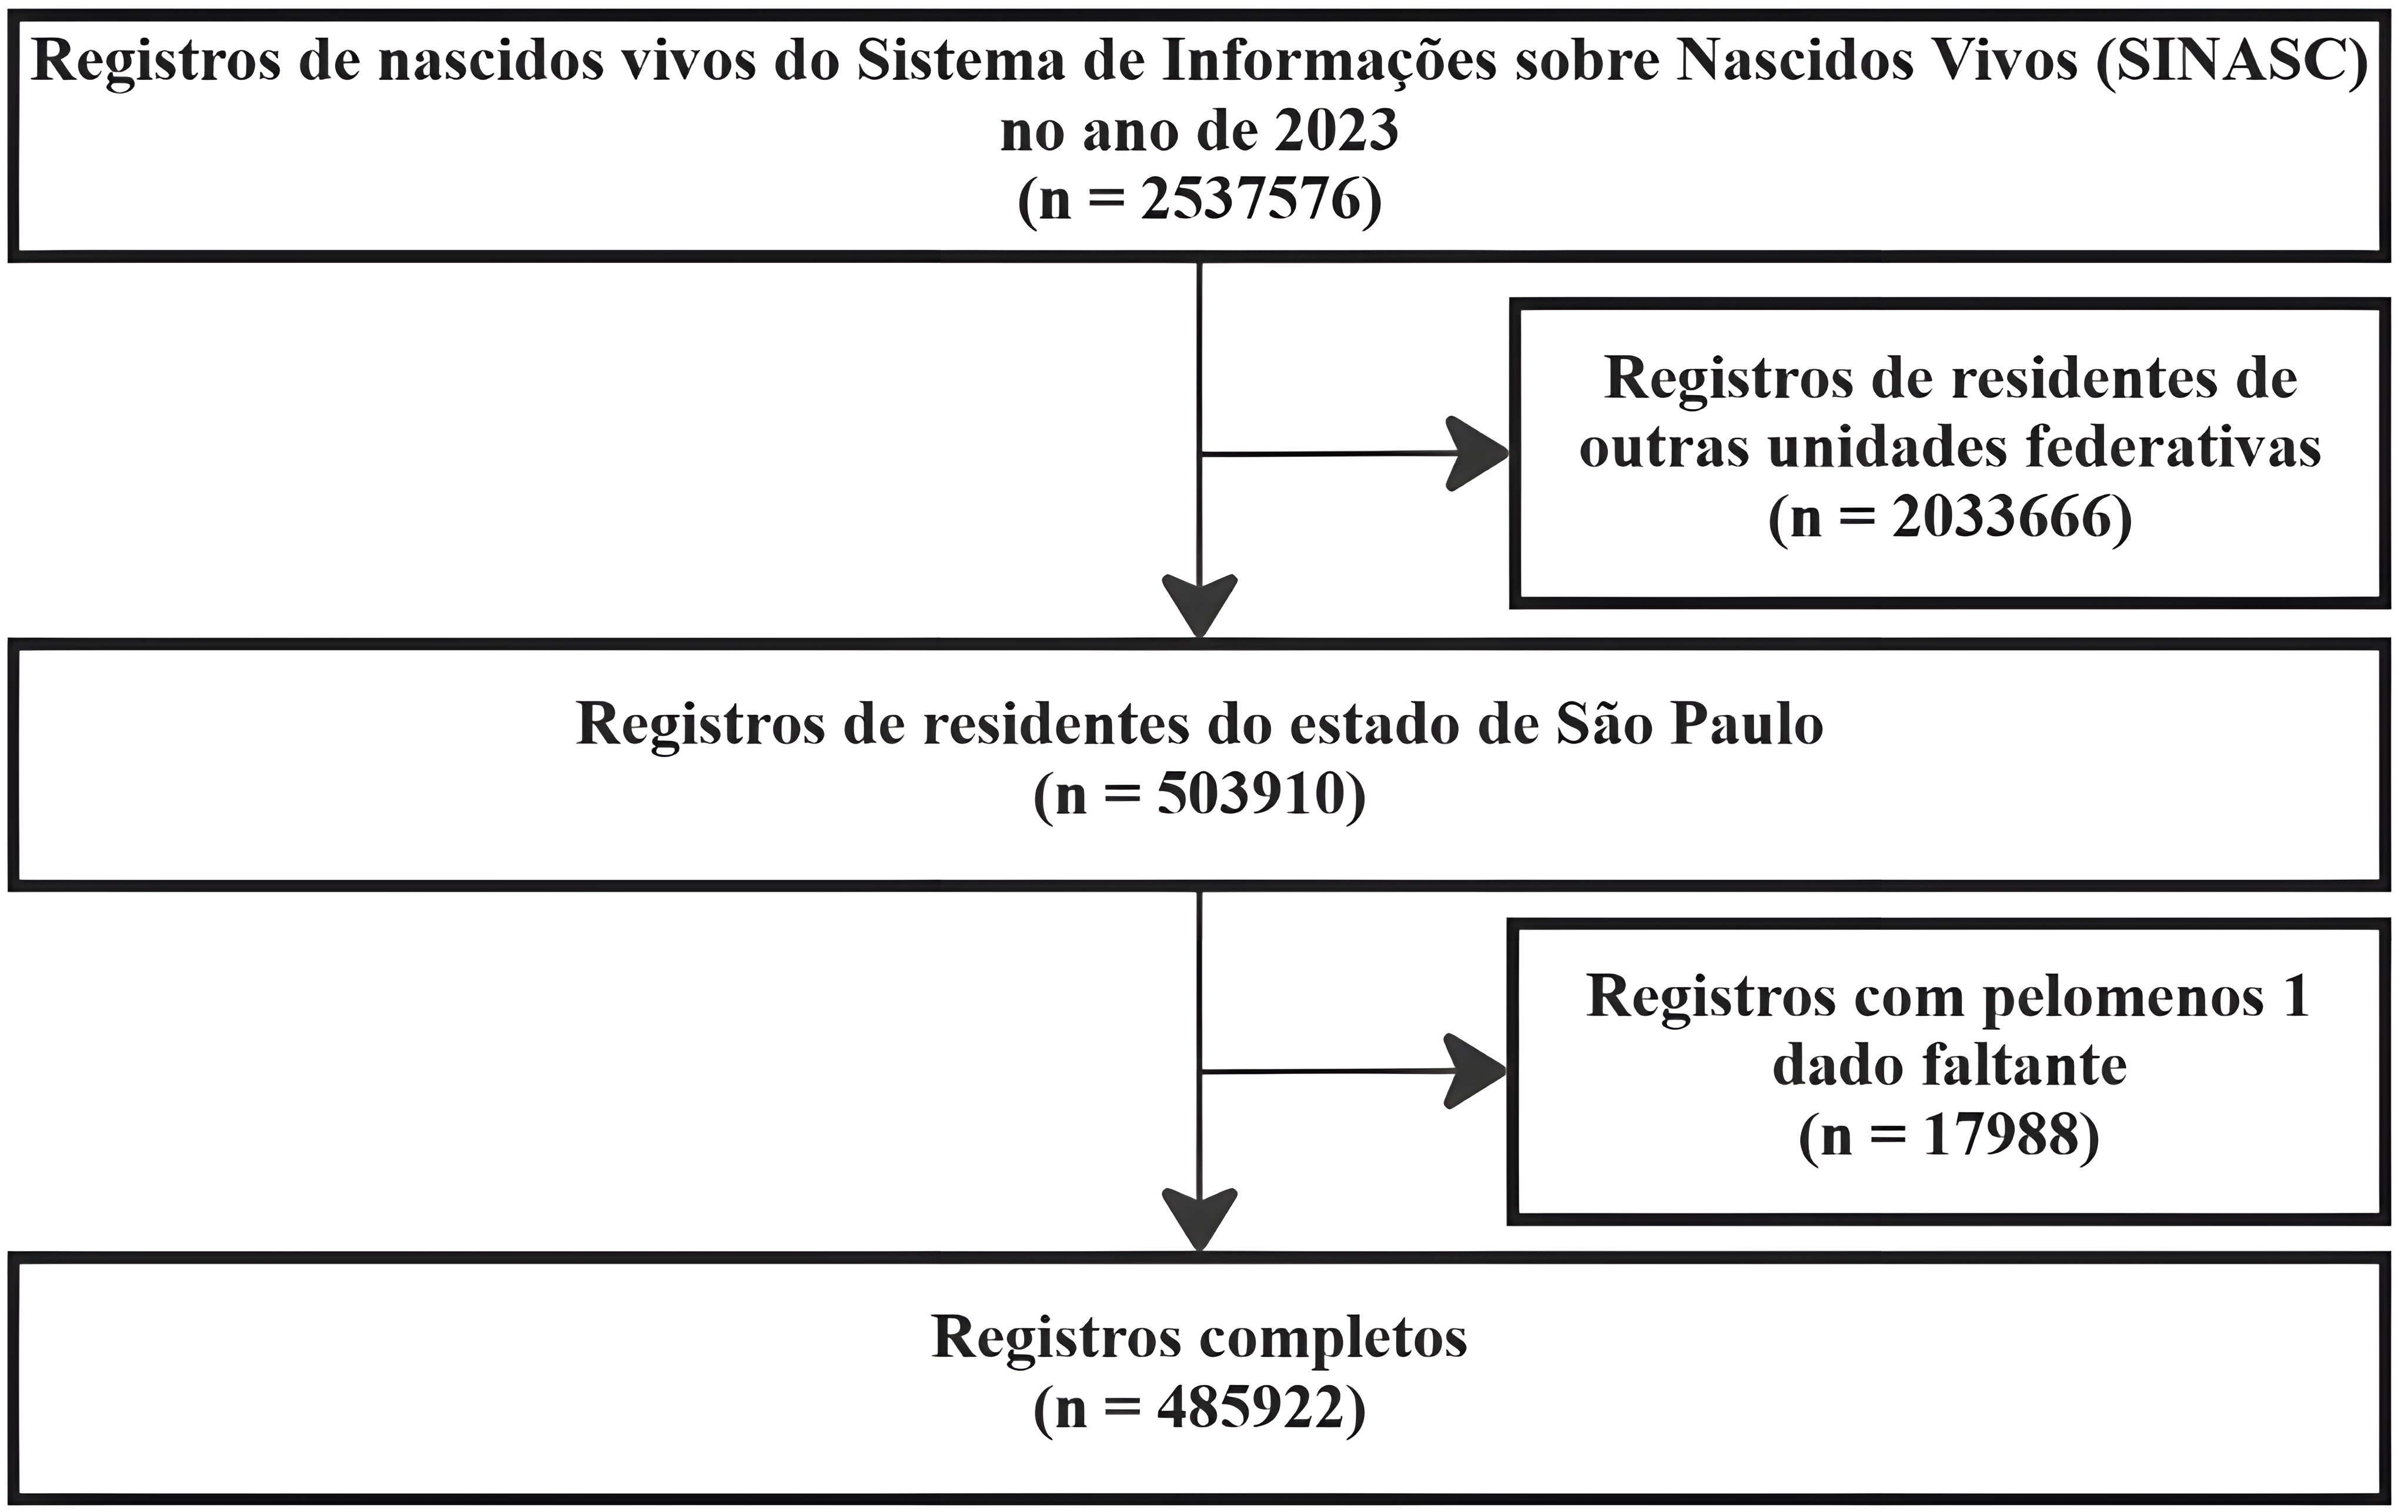
\includegraphics[width=0.8\linewidth]{figuras/flux_nascidos_vivos.png}
  \fonte{Fonte: figura elaborada pelo autor.}
  \label{fig:fluxograma-sinasc}
\end{figure}

\subsection{Variáveis abordadas e dados faltantes}

Foram inicialmente selecionadas 23 variáveis das bases de dados sendo consideradas, 
sendo 11 exclusivas do SINASC, 1 exclusiva do SIM-DOFET e 11 variáveis existentes em 
ambas. Além dessas, foi construída uma variável regional referente à RRAS de residência, 
obtida a partir do município de residência da mãe. As descrições das variáveis são 
apresentadas na Tabela \ref{fig:tabela-variaveis}.

%------------------------ Tabela com a lista das variáveis
\begin{table}[H]
    \centering
    \caption{Lista das variáveis abordadas no estudo.}
    \label{tab:variables}
    
    \small
    \renewcommand{\arraystretch}{1.05}
    \begin{tabular}{@{} L{3cm} L{7cm} L{3cm} @{}} 
        % Linha superior mais espessa
        \specialrule{0.12em}{0pt}{0pt}
        
        % CABEÇALHO: VARIÁVEIS NUMÉRICAS
        \multicolumn{1}{c}{\textbf{Variáveis numéricas}} &
        \multicolumn{1}{c}{\textbf{Descrição}} &
        \multicolumn{1}{c}{\textbf{Fonte}} \\
        \specialrule{0.12em}{0pt}{0pt}
        
        % Numéricas 
        \texttt{semagestac} &
        Número de semanas de gestação. &
        Ambos datasets \\
        
        \texttt{codmunres} &
        Código do município de residência da mãe. &
        Ambos datasets \\
        
        \texttt{idademae} &
        Idade da mãe em anos. &
        Ambos datasets \\
        
        \texttt{qtdfilvivo} &
        Número de filhos vivos anteriores (nascidos vivos). &
        Ambos datasets \\
        
        \texttt{qtdfilmort} &
        Número de filhos mortos anteriores (óbito fetal). &
        Ambos datasets \\
        
        \texttt{peso} &
        Peso ao nascer em gramas. &
        Ambos datasets \\
        
        \texttt{apgar5} &
        Índice de Apgar no quinto minuto (0 a 10). &
        SINASC \\
        
        \texttt{qtdgestant} &
        Número total de gestações anteriores. &
        SINASC \\
        
        \texttt{qtdpartnor} &
        Número de partos vaginais anteriores. &
        SINASC \\
        
        \texttt{qtdpartces} &
        Número de partos cesáreos anteriores. &
        SINASC \\
        
        \texttt{mesprenat} &
        Mês de gestação em que se iniciou o pré-natal. &
        SINASC \\
        
        % Separador entre blocos
        \specialrule{0.12em}{6pt}{0pt}
        
        % CABEÇALHO: VARIÁVEIS CATEGÓRICAS
        \multicolumn{1}{c}{\textbf{Variáveis categóricas}} &
        \multicolumn{1}{c}{\textbf{Descrição}} &
        \multicolumn{1}{c}{\textbf{Fonte}} \\
        \specialrule{0.12em}{0pt}{0pt}
        
        %Categóricas
        \texttt{sexo} &
        Sexo do feto (masculino ou feminino). &
        Ambos datasets \\
        
        \texttt{escmae2010} &
        Escolaridade da mãe (sem escolaridade, primeiro fundamental, segundo
        fundamental, médio, superior incompleto ou superior completo). &
        Ambos datasets \\
        
        \texttt{gravidez} &
        Tipo de gravidez (única, dupla, trípla ou mais). &
        Ambos datasets \\
        
        \texttt{parto} &
        Tipo de parto (vaginal ou cesáreo). &
        Ambos datasets \\
        
        \texttt{lococornasc} &
        Local de ocorrência do nascimento ou óbito (hospital, outros
        estabelecimentos de saúde, domicílio ou outros). &
        Ambos datasets \\
        
        \texttt{obitoparto} &
        Momento do óbito em relação ao parto (antes ou durante). &
        SIM-DOFET \\
        
        \texttt{consultas} &
        Número de consultas pré-natal registradas (nenhuma, 1 a 3, 4 a 6 ou 7 e mais). &
        SINASC \\
        
        \texttt{idanomal} &
        Anomalia identificada (sim ou não). &
        SINASC \\
        
        \texttt{racacormae} &
        Raça/cor da mãe (branca, preta, amarela, parda ou indígena). &
        SINASC \\
        
        \texttt{sttrabpart} &
        Trabalho de parto induzido (sim, não ou não se aplica). &
        SINASC \\
        
        \texttt{stcesparto} &
        Cesárea ocorreu antes do trabalho de parto iniciar (sim, não ou não se
        aplica). &
        SINASC \\
        
        \texttt{paridade} &
        Define se é a primeira gravidez ou se teve mais de uma (nulípara ou
        multípara). &
        SINASC \\
        
        \texttt{rras\_nome} &
        RRAS de residência, definida a partir do município de residência da mãe. &
        -- \\
        
        % Linha inferior padrão
        \bottomrule
    \end{tabular}
\fonte{Variáveis organizadas por tipo, com descrição e informação sobre qual é a
base de dados de origem. Fonte: tabela elaborada pelo autor.}
\label{fig:tabela-variaveis}
\end{table}

A Tabela \ref{fig:tabela-dados-faltantes} lista a quantidade de dados faltantes
nas variáveis de cada base considerada. As porcentagens foram calculadas em relação 
ao total de registros de cada variável. Além disso, ambas as bases de dados possuem 
variáveis com categorias identificadas como \emph{Ignorado}, as quais também foram 
consideradas como parte dos dados faltantes. É possível notar que, em geral, nenhuma 
variável do SINASC apresenta mais de 2\% de dados faltantes. Por outro lado, a base 
do SIM-DOFET apresenta a variável \texttt{escmae2010} com 16\% de dados faltantes 
(406 registros \emph{Ignorado} + 307 faltantes), enquanto as demais variáveis 
apresentam porcentagens inferiores a 7\%.

%------------------------ Tabela com a porcentagem de dados faltantes
\begin{table}[H]
    \centering
    \caption{Proporção de dados faltantes por variável nas bases SIM-DOFET e SINASC.}
    \label{tab:missing}
    
    \begin{tabular}{@{} L{4cm} C{4cm} C{4cm} @{}} 
        % Linha superior mais espessa
        \specialrule{0.16em}{0pt}{0pt}
        
        % CABEÇALHO: VARIÁVEIS NUMÉRICAS
        \multicolumn{1}{c}{\textbf{Variáveis numéricas}} &
        \multicolumn{1}{c}{\textbf{SIM-DOFET (\% faltante)}} &
        \multicolumn{1}{c}{\textbf{SINASC (\% faltante)}} \\
        \specialrule{0.16em}{0pt}{0pt}
        
        % Numéricas
        \texttt{semagestac}  & 2,16\%  & 0,10\%  \\
        \texttt{codmunres}   & 0,00\%  & 0,00\%  \\
        \texttt{idademae}    & 4,74\%  & 0,00\%  \\
        \texttt{qtdfilvivo}  & 4,52\%  & 0,22\%  \\
        \texttt{qtdfilmort}  & 6,36\%  & 0,33\%  \\
        \texttt{peso}        & 3,84\%  & 0,00\%  \\
        \texttt{apgar5}      & --      & 0,36\%  \\
        \texttt{qtdgestant}  & --      & 0,17\%  \\
        \texttt{qtdpartnor}  & --      & 0,27\%  \\
        \texttt{qtdpartces}  & --      & 0,22\%  \\
        \texttt{mesprenat}   & --      & 1,46\%  \\
        
        % Separador entre blocos (linha forte)
        \specialrule{0.16em}{0pt}{0pt}
        
        % CABEÇALHO: VARIÁVEIS CATEGÓRICAS
        \multicolumn{1}{c}{\textbf{Variáveis categóricas}} &
        \multicolumn{1}{c}{\textbf{SIM-DOFET (\% faltante)}} &
        \multicolumn{1}{c}{\textbf{SINASC (\% faltante)}} \\
        \specialrule{0.16em}{0pt}{0pt}
        
        % Categóricas
        \texttt{sexo}        & 2,59\%  & 0,02\%  \\
        \texttt{escmae2010}  & 16,00\% & 0,14\%  \\
        \texttt{gravidez}    & 1,26\%  & 0,02\%  \\
        \texttt{parto}       & 1,87\%  & 0,01\%  \\
        \texttt{lococornasc} & 0,07\%  & 0,00\%  \\
        \texttt{obitoparto}  & 4,18\%  & --      \\
        \texttt{consultas}   & --      & 0,17\%  \\
        \texttt{idanomal}    & --      & 0,41\%  \\
        \texttt{racacormae}  & --      & 0,31\%  \\
        \texttt{sttrabpart}  & --      & 0,23\%  \\
        \texttt{stcesparto}  & --      & 0,68\%  \\
        \texttt{paridade}    & --      & 0,00\%  \\
        \texttt{rras\_nome}  & --      & --      \\
        
        % Linha inferior padrão (mais fina que as de cabeçalho)
        \bottomrule
    \end{tabular}
    
    \vspace{2pt}
    \fonte{Porcentagens de dados faltantes calculadas em relação ao total da
    variável, onde dados de categoria \emph{Ignorado} estão inclusos no cálculo.
    Fonte: tabela elaborada pelo autor.}
    \label{fig:tabela-dados-faltantes}
\end{table}

Após essas verificações, optou-se por conduzir as análises apenas com os casos 
válidos, ou seja, registros com informação disponível para as variáveis sendo 
utilizadas. Essa escolha foi adotada porque as proporções de ausência foram baixas 
na maior parte das variáveis e porque imputar valores em variáveis, como idade 
gestacional e características maternas e obstétricas, exigiria pressupostos 
adicionais que não são o foco deste estudo. A principal ressalva é a variável 
referente à escolaridade materna no SIM-DOFET, que apresentou maior proporção de 
ausência, por isso, seus resultados devem ser interpretados com cautela.

\section{Análise}

\subsection{Construção da base de análise e definição dos desfechos}

As análises foram conduzidas em etapas, acompanhando o processo de construção da 
base utilizada nas análises. Primeiro, as bases SIM-DOFET e SINASC foram preparadas
separadamente. Depois, as variáveis comuns às duas bases foram padronizadas e
unidas em uma base única, permitindo analisar o tempo até o parto considerando dois 
possíveis desfechos: óbito fetal e nascimento vivo. As variáveis exclusivas de cada 
base e os indicadores regionais por RRAS foram analisados em blocos próprios.

A unidade de análise foi a gestação registrada nas bases de dados. O tempo de 
seguimento foi definido pela idade gestacional em semanas, representada por 
$T_i$, correspondente à variável \texttt{semagestac}. Na base conjunta, foi 
definida uma variável de causa do desfecho, $\delta_i$, com $\delta_i=1$ para 
óbito fetal e $\delta_i=2$ para nascimento vivo. Como as bases utilizadas são 
formadas por registros de eventos já ocorridos, não houve censura à direita 
no sentido clássico de análise de sobrevivência. Todas as gestações incluídas 
na base conjunta apresentaram encerramento observado, seja por óbito fetal 
ou por nascimento vivo. Assim, a censura utilizada nas curvas de Kaplan-Meier 
tem intuito analítico, onde, ao estimar a curva para uma causa específica, 
o desfecho concorrente é tratado como censura apenas para permitir a descrição 
separada do tempo até cada evento. Na análise de riscos competitivos, por sua vez, 
os dois desfechos são mantidos como causas observadas do encerramento da gestação, 
sem censura.

\subsection{Descrição dos dados e recategorização das variáveis}

A descrição inicial dos dados foi feita respeitando a natureza das variáveis. 
As variáveis numéricas foram descritas por média, desvio padrão, mediana, primeiro 
quartil e terceiro quartil. Nas variáveis categóricas, além das frequências 
absolutas e percentuais, também foram calculadas medidas resumo da idade gestacional 
dentro de cada categoria. Como essa variável pode apresentar assimetria, especialmente 
nos óbitos fetais e nos grupos com maior concentração de prematuridade, foi priorizada 
a mediana acompanhada do intervalo interquartílico (Q1--Q3) para a interpretação 
do tempo gestacional. A média e o desvio padrão foram usados como medidas 
complementares apenas quando ajudaram a evidenciar pequenos deslocamentos entre 
grupos, principalmente em situações nas quais as medianas foram iguais. Nesses 
casos, os valores foram descritos como média $\pm$ desvio padrão, com a mediana 
apresentada entre parênteses quando necessário.

Algumas variáveis foram recategorizadas para facilitar a interpretação e evitar 
categorias muito fragmentadas. A idade materna (Faixa etária materna) foi agrupada 
em menores de 20 anos, 20 a 34 anos e 35 anos ou mais, pois os extremos de idade 
materna são descritos na literatura como grupos de maior risco para desfechos 
gestacionais desfavoráveis \cite{Victor2025PretermBrazil,ACOG2020Stillbirth}. A escolaridade 
materna foi agrupada em Baixa (sem escolaridade ou primeiro fundamental), Média 
(segundo fundamental ou ensino médio) e Alta (superior incompleto ou completo), mantendo 
a interpretação social dessa variável e sua relação com desigualdades no pré-natal, 
na prematuridade e no óbito fetal \cite{Marques2026FetRiskS,Silva2026PrenatalInequities}. 
A variável referente à gravidez (Tipo de gravidez) foi classificado como única ou múltipla, 
e o local de ocorrência foi agrupado em hospital ou outros locais, de modo a preservar 
categorias com sentido assistencial e obstétrico \cite{ACOG2020Stillbirth,Sun2018}. 

O peso ao nascer foi classificado em menor que 2.500 g, 2.500 g a 3.999 g e igual 
ou superior a 4.000 g, separando baixo peso, faixa intermediária e pesos elevados, 
já que o crescimento fetal e as condições placentárias são marcadores importantes no 
estudo dos desfechos perinatais \cite{gardosi2013maternal,smith2007stillbirth,pinar2014placental}. 
As variáveis referentes a filhos vivos e filhos mortos previamente foram dicotomizadas 
em ausência ou presença desse antecedente, pois o histórico obstétrico desfavorável é 
apontado como fator relevante para o óbito fetal \cite{Lawn2016,ACOG2020Stillbirth,Sun2018}. 
Nas variáveis exclusivas do SINASC, o Apgar no quinto minuto foi categorizado em 
maior que 7 e igual ou inferior a 7, o início do pré-natal foi agrupado por trimestre 
(primeiro ao terceiro trimestre) e as variáveis de histórico obstétrico foram 
organizadas em categorias de presença ou ausência quando apropriado, preservando 
a leitura assistencial das informações disponíveis na Declaração de Nascido Vivo 
e a importância do acompanhamento pré-natal \cite{ministerioSaudeDNV2022,Silva2026PrenatalInequities}.

\subsection{Análise de sobrevivência e riscos competitivos}

As variáveis exclusivas de cada base foram avaliadas separadamente. No SIM-DOFET,
como todos os registros correspondem a óbitos fetais, a análise de Kaplan-Meier
descreveu a distribuição empírica da idade gestacional até o óbito fetal. No
SINASC, como todos os registros correspondem a nascimentos vivos, a mesma lógica
foi usada para descrever a distribuição da idade gestacional até o nascimento
vivo. Nesses dois casos isoladamente, não há evento competitivo dentro da base em
análise, portanto, os gráficos e testes descrevem diferenças na distribuição do
tempo gestacional entre categorias da variável avaliada.

Na análise de sobrevivência, a função de sobrevivência foi definida como $S(t)=P(T>t)$, 
ou seja, a probabilidade de a gestação ainda não ter apresentado o desfecho de interesse 
até a idade gestacional $t$. As curvas de Kaplan-Meier foram usadas para descrever 
essa função ao longo das semanas de gestação. Na base conjunta, as curvas foram 
estimadas sob duas perspectivas: óbito fetal como evento de interesse, censurando 
os nascimentos vivos, e nascimento vivo como evento de interesse, censurando os 
óbitos fetais. A comparação global entre curvas foi feita pelo teste de Log-rank, 
cuja estatística foi apresentada como $\chi^2$, com graus de liberdade definidos 
pelo número de categorias menos um.

Como o problema principal envolve dois desfechos mutuamente excludentes, também
foram estimadas funções de incidência acumulada (CIF) no contexto de riscos 
competitivos. Para a causa $k$, a CIF foi definida na Equação \ref{eq:cif-causa}:
\begin{equation}
\lequation{Função de incidência acumulada por causa}
\label{eq:cif-causa}
C_k(t)=P(T_i\leq t,\delta_i=k),
\end{equation}
ou seja, a probabilidade acumulada de ocorrência da causa $k$ até a idade
gestacional $t$, considerando a presença da causa concorrente. As funções 
de incidência acumulada foram estimadas para as variáveis comuns às duas bases 
e comparadas entre grupos pelo teste de Gray \cite{gray1988class}. 
Para a apresentação das CIF no texto, foram extraídos valores nas semanas 30, 35 
e 40. Esses pontos foram escolhidos por permitirem uma melhor leitura obstétrica: 
30 semanas representa prematuridade acentuada, 35 semanas se aproxima da faixa 
de prematuridade tardia e 40 semanas representa o termo. As medianas, intervalos 
interquartílicos, médias e desvios padrão citados junto aos gráficos correspondem 
à distribuição observada da idade gestacional em cada grupo, e não a uma estimativa 
obtida diretamente das curvas de Kaplan-Meier ou das CIF.

\subsection{Análise regional}

Para as análises regionais, os registros foram classificados segundo a divisão 
oficial em 18 Redes Regionais de Atenção à Saúde (RRAS) do estado de São Paulo 
usando o código do município de residência da mãe. Os mapas foram construídos 
a partir do shapefile municipal do estado de São Paulo, e foi realizado a agregação 
das geometrias municipais para o nível das RRAS. Também foi utilizada a população 
municipal do Censo 2022 para calcular indicadores populacionais por RRAS.

Para facilitar a interpretação, os resultados regionais foram pensados em três 
grupos de medidas. O primeiro grupo descreveu o volume de eventos em cada RRAS, 
por meio das contagens de óbitos fetais e de nascidos vivos e da participação 
percentual de cada RRAS no total estadual desses eventos. Esses percentuais 
indicam quanto cada RRAS contribuiu para o total observado no estado, e não devem 
ser interpretados como medida de risco. O segundo grupo reuniu indicadores com 
denominador regional explícito sendo, a razão de mortalidade fetal por 1.000 nascidos 
vivos e os nascidos vivos por 1.000 habitantes. A razão de mortalidade fetal foi 
calculada dividindo o número de óbitos fetais pelo número de nascidos vivos da 
RRAS e multiplicando o resultado por 1.000. O indicador de nascidos vivos por 
1.000 habitantes foi calculado dividindo o número de nascidos vivos pela 
população residente da RRAS e multiplicando o resultado por 1.000. O terceiro 
grupo descreveu a prematuridade entre nascidos vivos, definida como idade 
gestacional inferior a 37 semanas entre os registros com informação válida de 
idade gestacional. Como a definição da base de análise final considerou apenas 
registros completos nas variáveis de interesse, incluindo a RRAS de residência, 
todos os registros analisados foram agrupados por RRAS.

\subsection{Critérios de significância e interpretação}

Foi adotado nível de significância de 5\% para os testes estatísticos. Assim,
valores de $p<0{,}05$ foram considerados indicativos de diferença estatisticamente 
significativa entre curvas ou grupos. Nas tabelas, os símbolos *** e ** foram 
utilizados para representar, respectivamente, $p<0{,}001$ e $p<0{,}01$. Valores-p 
sem esses símbolos foram apresentados numericamente quando necessário. Em todas as 
interpretações, os resultados dos testes foram avaliados em conjunto com os gráficos, 
as frequências e a magnitude das diferenças observadas, considerando que o grande 
tamanho amostral pode tornar estatisticamente significativas diferenças pequenas 
do ponto de vista prático.

\section{Desenvolvimento do modelo}

\subsubsection*{Desenvolvimento da abordagem de riscos competitivos -- sem
considerar fragilidade compartilhada}

Seja $T_i$ o tempo até o parto da $i$-ésima observação. O parto pode ocorrer por
duas causas: óbito fetal ou nascimento vivo. Seja $\delta_i$ o indicador da causa
do parto, com $P(\delta_i=k)=p_k$, em que $k=1$ (óbito fetal) e $k=2$
(nascimento vivo), com $p_1+p_2=1$.

Seja $F_k(t)=P(T_{ik}\leq t| \delta_i=k)$, em que $F_1(\cdot)$ e
$F_2(\cdot)$ são próprias, e $T_{ik}$ é o tempo até o parto pela causa $k$.
Além disso, seja $T_i=T_{ik}$ em $\{\delta_i=k\}$. A distribuição marginal
correspondente é dada pela Equação \ref{eq:distribuicao-marginal-tempo-parto}:

\begin{equation}
\lequation{Distribuição marginal do tempo até o parto}
\label{eq:distribuicao-marginal-tempo-parto}
\begin{aligned}
F(t)&=P(T_i\leq t)=P(T_{i1}\leq t| \delta_i=1)P(\delta_i=1)
+P(T_{i2}\leq t| \delta_i=2)P(\delta_i=2)\\
&=p_1F_1(t)+p_2F_2(t).
\end{aligned}
\end{equation}

A função de risco causa-específica da $k$-ésima causa é dada pela Equação \ref{eq:risco-causa-especifica}:
\begin{equation}
\lequation{Risco causa-específico}
\label{eq:risco-causa-especifica}
\lambda_k(t)\,dt
=P(T_i\in(t,t+dt),\text{ causa } k| T_i>t),
\end{equation}
e
\[
\lambda(t)=\lambda_1(t)+\lambda_2(t)=\frac{F'(t)}{1-F(t)}.
\]

Ainda,
\[
p_k=P(\delta_i=k)
=\int_0^\infty
\frac{P(t\leq T_{ik}\leq t+\Delta,\delta_i=k)}{\Delta}\,dt
=\int_0^\infty \lambda_k(t)S(t)\,dt.
\]

A função distribuição condicional dado a causa $k$ é:
\[
F_k(t)=P(T_{ik}\leq t| \delta_i=k)
=\frac{P(T_{ik}\leq t,\delta_i=k)}{P(\delta_i=k)}
=\frac{\int_0^t \lambda_k(u)S(u)\,du}{p_k}.
\]

Consequentemente,
\[
dF_k(t)=\frac{\lambda_k(t)S(t)}{p_k}.
\]

Assim,
\[
\lambda_k(t)=\frac{p_kf_k(t)}{S(t)},
\]
sendo $f_k(t)=\frac{dF_k(t)}{dt}
=\lim_{\Delta\to0}
\frac{P(t\leq T_{ik}<t+\Delta| \delta_i=k)}{\Delta}$.

Define-se uma distribuição para $F_k(t)$, indexada por $\theta$, e então obtém-se
$f_k(t)=dF_k(t)$. A função de verossimilhança para $\theta$ é apresentada na Equação \ref{eq:verossimilhanca-sem-fragilidade} \cite{maller2002}:
\begin{equation}
\lequation{Verossimilhança sem fragilidade compartilhada}
\label{eq:verossimilhanca-sem-fragilidade}
L(\theta)\propto
\prod_{i=1}^{n}
\left[p_1f_1(t_i)\right]^{I(\delta_i=1)}
\left[p_2f_2(t_i)\right]^{I(\delta_i=2)}.
\end{equation}

\subsubsection*{Desenvolvimento dentro do $j$-ésimo cluster}

Seja $T_{ji}$ o tempo até o parto da $i$-ésima observação no $j$-ésimo cluster,
para $i=1,\ldots,n_j$ e $j=1,2,\ldots,R$, com $R$ sendo o número de clusters
(RRAS). Seja $\delta_{ji}$ o indicador da causa do parto, com
$P(\delta_{ji}=k)=p_k$, onde $k=1$ (óbito fetal) e $k=2$ (nascimento vivo),
com $p_1+p_2=1$.

Para cada cluster (aqui, cada RRAS), seja $Z_j$ uma variável de fragilidade
compartilhada representando a vulnerabilidade latente geral da região $j$,
comum a ambas as causas de falha. Essa variável atua como um efeito aleatório
multiplicativo, capturando heterogeneidade regional não observada e induzindo
dependência entre indivíduos pertencentes ao mesmo cluster.

Em termos práticos, todos os indivíduos na mesma RRAS compartilham o mesmo valor
de fragilidade $Z_j$, independentemente da causa, introduzindo correlação entre
seus tempos de falha. Essa especificação compartilhada assume que os fatores
estruturais, organizacionais e ambientais que tornam uma região vulnerável atuam
de forma semelhante tanto no risco de óbito fetal quanto no momento do nascimento
vivo, uma suposição parcimoniosa e defensável dado o número limitado de RRAS
($R=18$). Fragilidades causa-específicas são consideradas como análise de
sensibilidade. Assim, $Z_j$ modela explicitamente tanto a heterogeneidade regional
não explicada (diferenças entre clusters não capturadas pelas covariáveis
observadas) quanto a correlação intracluster.

Além disso, seja $\mathbf{x}_{kji}$ o vetor de covariáveis do $i$-ésimo indivíduo no
$j$-ésimo cluster para a $k$-ésima causa, e seja $\mathbf{X}_{kj}$ a matriz de covariáveis
dos $n_j$ indivíduos no cluster $j$.

A distribuição conjunta de $(T_j,\delta_j)$ condicional a $Z_j$, $\mathbf{X}_{1j}$ e
$\mathbf{X}_{2j}$ para o $j$-ésimo cluster é dada por:
\[
\begin{aligned}
&P\left(
\bigcap_{i=1}^{n_j}\{T_{ji}\in(t_{ji},t_{ji}+\Delta),\delta_{ji}=k_i\}
| Z_j,\mathbf{X}_{1j},\mathbf{X}_{2j}
\right)\\
&=\prod_{i=1}^{n_j}
P(T_{ji}\in(t_{ji},t_{ji}+\Delta),\delta_{ji}=k_i
| Z_j,\mathbf{x}_{1ji},\mathbf{x}_{2ji})\\
&=\prod_{i=1}^{n_j}
P(T_{ji}\in(t_{ji},t_{ji}+\Delta)|
\delta_{ji}=k_i,Z_j,\mathbf{x}_{1ji},\mathbf{x}_{2ji})
P(\delta_{ji}=k_i| Z_j,\mathbf{x}_{1ji},\mathbf{x}_{2ji})
\end{aligned}
\]
com $k_i=1,2$, para $i=1,\ldots,n_j$. Assume-se que os tempos até o parto dos
indivíduos dentro do mesmo cluster são independentes condicionalmente à variável
de fragilidade. Portanto, obtém-se a forma fatorada apresentada na Equação \ref{eq:distribuicao-condicional-cluster}:
\begin{equation}
\lequation{Distribuição conjunta condicional no cluster}
\label{eq:distribuicao-condicional-cluster}
\begin{aligned}
&P\left(
\bigcap_{i=1}^{n_j}\{T_{ji}\in(t_{ji},t_{ji}+\Delta),\delta_{ji}=k_i\}
| Z_j,\mathbf{X}_{1j},\mathbf{X}_{2j}
\right)\\
&=
 \prod_{i=1}^{n_j}
 \left[f_1(t_{ji}| Z_j,\mathbf{x}_{1ji})p_{1ji}\right]^{I(\delta_{ji}=1)}
 \left[f_2(t_{ji}| Z_j,\mathbf{x}_{2ji})p_{2ji}\right]^{I(\delta_{ji}=2)}.
\end{aligned}
\end{equation}

Seja $\theta$ o vetor de parâmetros relacionado às distribuições de $F_1(\cdot)$
e $F_2(\cdot)$. A função de verossimilhança para $\theta$ é dada pela Equação \ref{eq:verossimilhanca-com-fragilidade}:
\begin{equation}
\lequation{Verossimilhança com fragilidade compartilhada}
\label{eq:verossimilhanca-com-fragilidade}
L(\Theta| D)=
\prod_{j=1}^{R}\prod_{i=1}^{n_j}
\left[f_1(t_{ji}| Z_j,\mathbf{x}_{1ji})p_{1ji}\right]^{I(\delta_{ji}=1)}
\left[f_2(t_{ji}| Z_j,\mathbf{x}_{2ji})p_{2ji}\right]^{I(\delta_{ji}=2)}.
\end{equation}

Aqui,
$D=\{(t_{ji},\delta_{ji},\mathbf{x}_{1ji},\mathbf{x}_{2ji}),i=1,\ldots,n_j,j=1,\ldots,R\}$
denota a amostra observada, em que $t_{ji}$ é o tempo gestacional até o parto,
$\delta_{ji}$ é o indicador de causa, e $\mathbf{x}_{1ji}$, $\mathbf{x}_{2ji}$ são os vetores de
covariáveis para as causas 1 e 2, respectivamente.

Seguindo a estrutura paramétrica de mistura de Maller e Zhou \cite{maller2002},
são usadas diretamente as densidades condicionais $f_k$. Especificamente,
assume-se que $T_{ji}|(\delta_{ji}=k,Z_{kj},\mathbf{x}_{kji})$ segue uma distribuição
Weibull com parâmetro de forma $\alpha_k$ e parâmetro de escala $\phi_{kji}$,
de modo que a densidade condicional é apresentada na Equação \ref{eq:densidade-weibull-condicional}:
\begin{equation}
\lequation{Densidade Weibull condicional}
\label{eq:densidade-weibull-condicional}
f_k(t| Z_{kj},\mathbf{x}_{kji})=\alpha_k\phi_{kji}^{\alpha_k}t^{\alpha_k-1}
\exp(-(\phi_{kji}t)^{\alpha_k}),
\end{equation}
em que o parâmetro de escala incorpora covariáveis individuais e a fragilidade
espacial no nível do cluster, conforme a Equação \ref{eq:escala-fragilidade-espacial}:
\begin{equation}
\lequation{Parâmetro de escala com fragilidade espacial}
\label{eq:escala-fragilidade-espacial}
\phi_{kji}=\exp\bigl(\mathbf{x}_{kji}^{\top}\bm{\beta}_k+w_j\bigr),\quad \exp(w_j)=Z_j.
\end{equation}

A função de sobrevivência condicional correspondente é dada pela Equação \ref{eq:sobrevivencia-condicional-causa}:
\begin{equation}
\lequation{Sobrevivência condicional por causa}
\label{eq:sobrevivencia-condicional-causa}
S_k(t| Z_{kj},\mathbf{x}_{kji})=\exp(-(\phi_{kji}t)^{\alpha_k}),
\end{equation}
e a função de sobrevivência marginal decorre da estrutura de mistura, conforme a Equação \ref{eq:sobrevivencia-marginal-mistura}:
\begin{equation}
\lequation{Sobrevivência marginal da mistura}
\label{eq:sobrevivencia-marginal-mistura}
S(t)=p_1S_1(t)+p_2S_2(t).
\end{equation}
O risco causa-específico é uma quantidade derivada dada pela Equação \ref{eq:risco-causa-especifica-derivado}:
\begin{equation}
\lequation{Risco causa-específico derivado do modelo}
\label{eq:risco-causa-especifica-derivado}
\lambda_{kji}(t)=p_{kji}f_k(t| Z_j,\mathbf{x}_{kji})/S_{ji}(t).
\end{equation}

A probabilidade da causa $p_{1ji}=P(\delta_{ji}=1)$ varia entre indivíduos por
meio de uma regressão logística em um vetor de covariáveis $\mathbf{z}_{ji}$, conforme a Equação \ref{eq:modelo-logistico-causa}:
\begin{equation}
\lequation{Modelo logístico para probabilidade da causa}
\label{eq:modelo-logistico-causa}
\operatorname{logit}(p_{1ji})=\mathbf{z}_{ji}^{\top}\bm{\gamma},
\qquad
p_{2ji}=1-p_{1ji},
\end{equation}
em que $\mathbf{z}_{ji}$ inclui variáveis relacionadas à probabilidade de óbito fetal
versus nascimento vivo (por exemplo, histórico obstétrico e tipo de gestação), e
$\bm{\gamma}$ é o vetor correspondente de coeficientes de regressão. Essa estrutura de
dois componentes separa a questão de qual desfecho ocorre (governada por
$\bm{\gamma}$) da questão de quando ele ocorre dado o desfecho (governada por
$\bm{\beta}_k$, $\alpha_k$ e $w_j$).

Para a fragilidade espacial, $\mathbf{w}=(w_1,\ldots,w_R)$ segue uma priori intrínseca
condicional autorregressiva (ICAR) baseada na matriz de adjacência $\mathbf{W}$ das RRAS 
\cite{besag1991, rueheld2005}. Usando a precisão $\tau$, a priori ICAR é definida na Equação \ref{eq:priori-icar}:
\begin{equation}
\lequation{Priori espacial ICAR}
\label{eq:priori-icar}
\pi(\mathbf{w}| \tau)\propto
\tau^{(R-1)/2}
\exp\left\{
-\frac{\tau}{2}\sum_{j\sim l}(w_j-w_l)^2
\right\}.
\end{equation}
A priori ICAR é imprópria (deficiente em posto), de modo que a identificabilidade
requer a restrição de soma zero $\sum_{j=1}^{R}w_j=0$.

Assim, a especificação das prioris é apresentada na Equação \ref{eq:prioris-parametros}:
\begin{equation}
\lequation{Especificação das prioris dos parâmetros}
\label{eq:prioris-parametros}
\bm{\beta}_k\sim N(\mathbf{0},\sigma^2_{\beta_k}\mathbf{I}),\quad
\alpha_k\sim \operatorname{Gamma}(a_{\alpha_k},b_{\alpha_k}),\quad
\tau\sim \operatorname{Gamma}(a_\tau,b_\tau),\quad
\bm{\gamma}\sim N(\mathbf{0},\sigma^2_\gamma \mathbf{I}).
\end{equation}

Seja $\Theta=(\bm{\beta}_1,\bm{\beta}_2,\alpha_1,\alpha_2,\bm{\gamma},\mathbf{w},\tau)$. A distribuição
a posteriori é dada pela Equação \ref{eq:posteriori}:
\begin{equation}
\lequation{Distribuição a posteriori}
\label{eq:posteriori}
\pi(\Theta| D)\propto
L(\Theta| D)\pi(\bm{\beta}_1)\pi(\bm{\beta}_2)\pi(\alpha_1)\pi(\alpha_2)
\pi(\bm{\gamma})\pi(\mathbf{w}| \tau)\pi(\tau).
\end{equation}

Essa formulação separa a composição de covariáveis (que tipos de gestações
ocorrem em cada região) da vulnerabilidade regional latente (fatores estruturais,
organizacionais ou não mensurados que tornam algumas RRAS sistematicamente
diferentes), fornecendo suporte direto ao planejamento de políticas direcionadas
regionalmente.

Os hiperparâmetros são especificados usando prioris fracamente informativas. Para
os vetores de regressão, são adotadas prioris Normais centradas com variância grande
para regularizar efeitos extremos enquanto preservam associações
epidemiologicamente plausíveis, ou seja, 
$\bm{\beta}_k\sim N(\mathbf{0},\sigma^2_{\beta_k}\mathbf{I})$ e
$\bm{\gamma}\sim N(\mathbf{0},\sigma^2_\gamma \mathbf{I})$. Para os parâmetros de forma e precisão,
são usadas prioris Gamma com hiperparâmetros fixos escolhidos para garantir
posteriores próprias e evitar concentração excessiva a priori. Análises de 
sensibilidade sobre valores alternativos de $(a_{\alpha_k},b_{\alpha_k})$ e
$(a_{\tau_k},b_{\tau_k})$ são conduzidas para avaliar a robustez da inferência
a posteriori \cite{gelman2013, simpson2017, riebler2016}.
